\documentclass[12pt, a4paper, simple]{eskdtext}

\usepackage{hyperref}
\usepackage{_env/gpi_global.env}
\usepackage{_env/gpi_report.env}
\usepackage{_sty/gpi_lst}
\usepackage{_sty/gpi_toc}
\usepackage{_sty/gpi_t}
\usepackage{_sty/gpi_p}
\usepackage{_sty/gpi_u}

% Переменные
\def \gpiDocNum {4}
\def \gpiTopicRep {План деления элементов автоматизированной системы обработки информации (АСОИ)
на части (очереди) для их последующей реализации}

% Код
% \ESKDletter{О}{Л}{Р}
% \def \gpiDocTypeNum {81}
% \def \gpiDocVer {00}
% \def \gpiCode {\ESKDtheLetterI\ESKDtheLetterII\ESKDtheLetterIII.\gpiStudentGroupName\gpiStudentGroupNum.\gpiStudentCard-0\gpiDocNum~\gpiDocTypeNum~\gpiDocVer}

\def \gpiDocTopic {Отчёт лабораторной работы №\gpiDocNum}

% колонтитулы
\usepackage{fancybox, fancyhdr}
\fancypagestyle{plain}
{
    \renewcommand{\footrulewidth}{0pt}          % Толщина отделяющей полоски снизу
    \renewcommand{\headrulewidth}{0pt}          % Толщина отделяющей полоски сверху
    \fancyhead[C]{ }                            % Коллонтитул сверху
    \fancyfoot[C]{\hfill\hfillстр. \thepage}    % Коллонтитул снизу
}

% Графа 1 (наименование изделия/документа)
% \ESKDcolumnI {\ESKDfontII \gpiTopic \\ \gpiDocTopic}

% Графа 2 (обозначение документа)
% \ESKDsignature {\gpiCode}

% Графа 9 (наименование или различительный индекс предприятия) задает команда
% \ESKDcolumnIX {\gpiDepartment}

% Графа 11 (фамилии лиц, подписывающих документ) задают команды
% \ESKDcolumnXIfI {\gpiStudentSurname}
% \ESKDcolumnXIfII {\gpiTeacherSurname}
% \ESKDcolumnXIfV {\gpiTeacherSurname}

\begin{document}
    \begin{ESKDtitlePage}
    \ESKDstyle{empty}
    \begin{center}
        \gpiMinEduRep \\
        \gpiEduRep \\
        \gpiKafRep \\
    \end{center}

    \vfill

    \begin{center}
        Тема: <<\gpiTopicRep>>
    \end{center}

    \vfill

    \begin{center}
        \textbf{\gpiDocTopic} \\
        по дисциплине \gpiDisciplineRep \\
    \end{center}

    \vfill

    \begin{flushright}
        \begin{minipage}[t]{7cm}
            Выполнил:\\
            \PageTitleStudentInfo
            \PageTitleDateField
            \hspace{0pt}

            Проверил:\\
            \PageTitleTeacherInfo
            \PageTitleDateField
        \end{minipage}
    \end{flushright}

    \vfill

    \begin{center}
        \PageTitleCity~\ESKDtheYear
    \end{center}
\end{ESKDtitlePage}

    \ESKDstyle{empty}
    \thispagestyle{plain}
    \pagestyle{plain}

    \begin{center}
        \textbf{\gpiDocTopic}
    \end{center}

    % = = = = = = = =
    \paragraph{} \textbf{Тема}: <<\gpiTopicRep>>

    \paragraph{} \textbf{Цель}:
    Формирование знаний и умений по планированию производства АСОИ по очереди.

    \paragraph{Деление АСОИ на очереди}

    \begin{figure}[!hp]
        \begin{minipage}{0.48\textwidth}
            \centering
            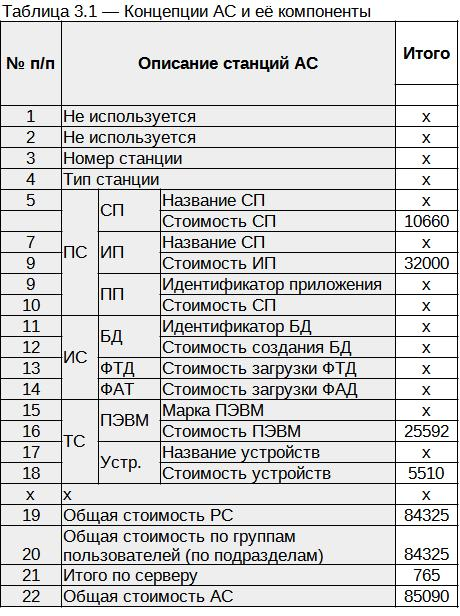
\includegraphics[height=8cm]
            {_docs/Таблица3-1КонцепцияАСИЕеКомпоненты.jpg}
            \caption{Концепция АС и её компоненты (из лаб1)}
        \end{minipage}
        \begin{minipage}{0.48\textwidth}
            \centering
            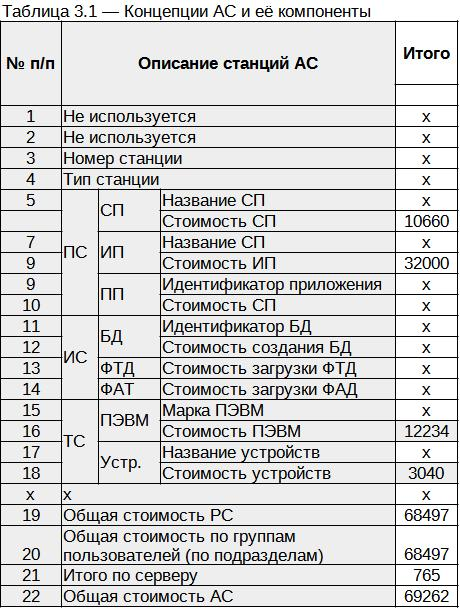
\includegraphics[height=8cm]
            {_docs/Таблица3-1КонцепцияАСИЕеКомпоненты__лаб2.jpg}
            \caption{Концепция АС и её компоненты (из лаб1)}
        \end{minipage}
     \end{figure}

    1. \underline{Определение плановой стоимости создания АСОИ} по формуле:
    
    <<Плановая стоимость АСОИ>> = <<Расчетная стоимость реализации АС>> * 1.2,
    где - Расчетная стоимость реализации АСОИ определяется из таблицы <<Концепция и ее компоненты>> (см. ЛР№2).
    
    <<Расчетная стоимость реализации АС>> = 69 262.00

    <<Плановая стоимость АСОИ>> = 69 262.00 * 1.2 = 83 114.40

    2. \underline{Определение стоимости реализации отдельной очереди АСОИ}.

    Расчет размера ресурсов выде­ляемых на каж­дую оче­редь АСОИ определяется на основе табл. Л.1 и Л.2
    (требования к реализации процесса «Реализация элементов»).
    Выделяемые финансовые ресурсы делятся на три части (на­пример, 20\%, 45\% и 35\% от плановой стоимо­сти реализации АСОИ)
    и опре­деля­ются их значе­ния для каждой очереди - Х1, Х2 и Х3.
    
    <<Плановая стоимость АСОИ>> = 83 114.40 руб.
    
    Тогда Х1, Х2 и Х3 имеют следующие значения:

    Х1 = 83 114.40 руб * 0.2 =16 622.88 руб.

    Х2 = 83 114.40 руб * 0.45 = 37 401.48 руб.
    
    Х3 = 83 114.40 руб * 0.35 = 29 090.04 руб.

    ФТД = Объём данных для загрузки (ФТД) (лаб1) = 6 600.00

    ФАД = Объём данных для загрузки (ФАД) (лаб1) = 10 168.00

    ФТД = Объём данных для загрузки файлов в БД (ФТД) (лаб1) = 24.75

    ФАД = Объём данных для загрузки файлов в БД (ФАД) (лаб1) = 38.13

    БД = Стоимость создания БД (лаб1) = 220.31

    3. \underline{Деление АСОИ на очереди}.
    Возможны следующие способы деления АСОИ на очереди:
    \begin{itemize}
        \item[-] Применение методов оптимизации для деления АСОИ на очереди,
        которые рассматрива­лись в рамках дисциплины «Системный анализ и исследование операций» [3].
        В качестве критерия оптимизации можно использовать время создания очередей и АСОИ в целом.
        Дан­ный способ используется для получения высокой оценки по КП!!!
        \item[-] «Подбор» возможного варианта деления АСОИ на очереди без учета критериев оптимиза­ции. 
    \end{itemize}

    Выбор способа деления АСОИ на части студент определяет самостоятельно.

    % \textbf{Второй способ деления АСОИ на части}.
    % Основные положения этого способа решения задачи следую­щие:
    % \begin{enumerate}
    %     \item[1.] Первоначальное определение элементов для первой очереди АСОИ:
    %     \item[1.1.] Выбор для реализации следующих элементов ТС: серверных РС;
    %     РС для экс­плуа­тацион­ного персонала; одной пользовательской РС
    %     (на основе анализа сетевого графика и плана реализации ПС).  
    %     \item[1.2.] Выбор для реализации  СП и ИП необходимых для РС перечисленных в п.1.1. 
    %     \item[1.3.] Выбор для реализации БД.
    %     \item[1.4.] Выбор для реализации элементов ПС для пользовательской РС, кот. опреде­лена в п.1.1. 
    %     \item[1.5.] Оценка стоимости первой очереди АСОИ. 
    %     \item[2.] Анализ стоимости первой очереди АСОИ:
    %     \item[-] Если стоимость первой очереди меньше запланированной,
    %     то возможно включение в пер­вую очередь для реализации следующих элементов
    %     (в рамках свободной стоимости для первой очереди): ФТД и/или ФАД; оборудования для пользователь­ских РС.
    %     При этом оценка стоимости первой очереди не должна превышать ее пла­новую стоимость.  
    %     \item[-] Если стоимость первой очереди выше плановой стоимости, то переход к п.3. 
    %     \item[3.] Уточнение стоимости очередей для АСОИ:
    %     \item[-] Зафиксировать рассчитанную стоимость для первой очереди,
    %     которая была полу­чена при вы­полнении действий в п.1- п.2.
    %     \item[-] Если стоимость первой очереди выше плановой, то разницу вычесть из стоимости второй очереди. 
    %     \item[-] Если стоимость первой очереди ниже плановой стоимости,
    %     то ее разницу добавить к стоимо­сти второй очереди. 
    %     \item[4.] Планирование реализации элементов для второй очереди.
    %     Реализуется подбор элемен­тов ТС, БД и ПС на основе сетевых графиков и планов их реализации
    %     и с учетом плано­вой стоимости для второй очереди.
    %     \item[5.] Анализ стоимости второй очереди (по аналогии с п.2).
    %     \item[6.] Уточнение стоимости второй очереди АСОИ (по аналогии с п.3).
    %     \item[7.] Реализация остальных очередей АСОИ (по аналогии с п.4 - п.6).	
    % \end{enumerate}

    % \textbf{Примечание}.
    % При делении АСОИ на части разрешается изменять значения показателей Х1, Х2 и Х3 в размере 5\%,
    % сохраняя постоянной общую плановую стоимость.

    % На рисунке 3.2 приведен пример деления АСОИ на две очереди (части).
    % Для наглядности струк­тура РС (ПЭВМ, уст­рой­ства, СП и ИП) на рисунке не изображены.

    % В данном подразделе представляются результаты деления элементов АСОИ на очереди в графи­ческой форме (в виде рисунка).

    \begin{figure}[ph!]
        \centering
        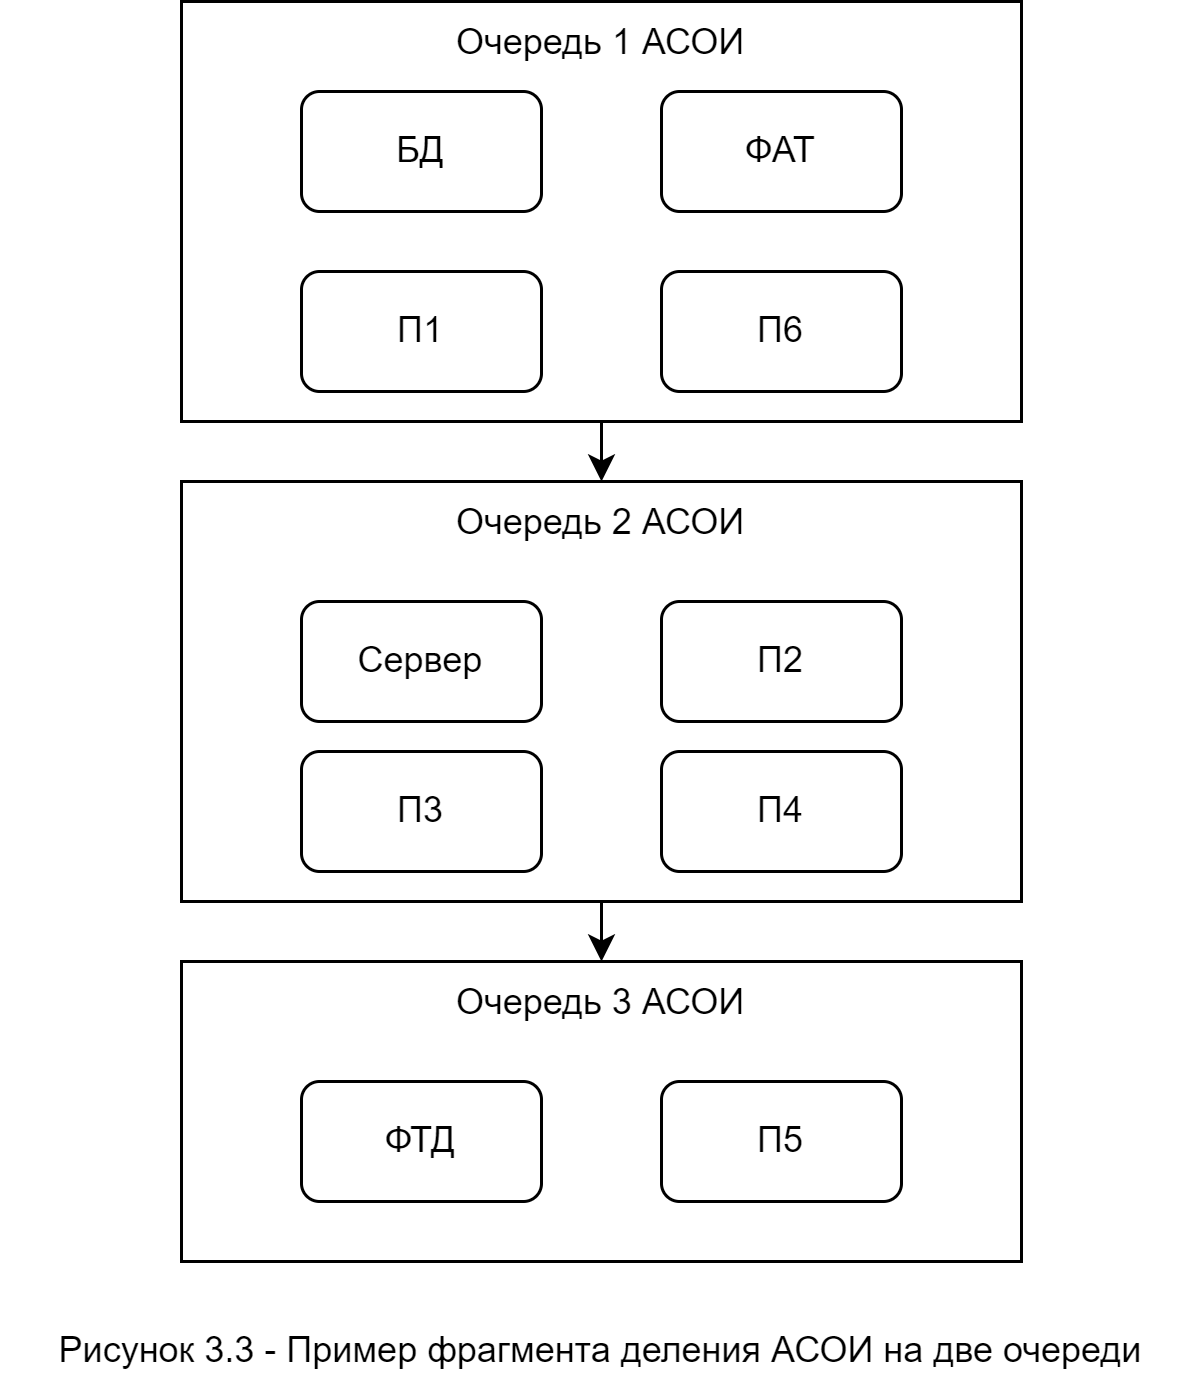
\includegraphics[width=12cm]
            {_docs/Рисунок3-3ПримерФрагментаДеленияАСОИНаДвеОчереди.png}
        \caption{Пример логической структуры ПС АСОИ}
    \end{figure}

    \newpage

    \begin{figure}[p!]
        \centering
        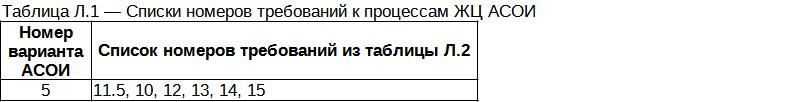
\includegraphics[]
            {_docs/ТаблицаЛ1СпискиНомеровТребованийКПроцессамЖЦАСОИ.jpg}
        \caption{Списки номеров требований к процессам ЖЦ АСОИ}
    \end{figure}

    \begin{figure}[p!]
        \centering
        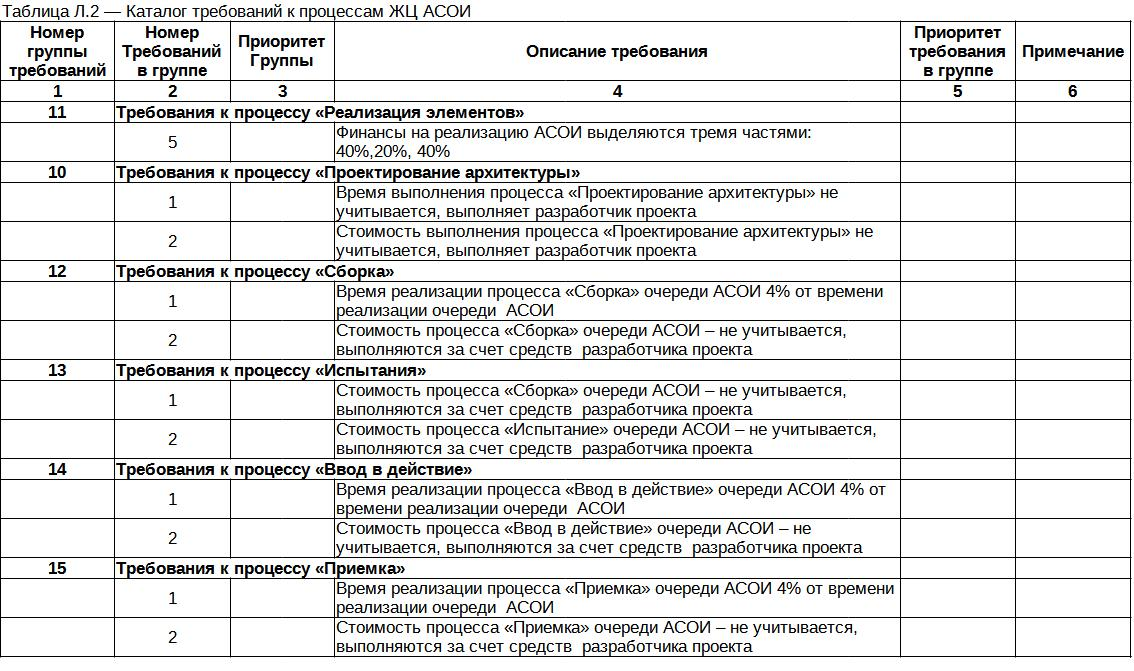
\includegraphics[width=16cm]
            {_docs/ТаблицаЛ2КаталогТребованийКПроцессамЖЦАСОИ.jpg}
        \caption{Каталог требований к процессам ЖЦ АСОИ}
    \end{figure}

    \newpage

    % \paragraph{Разработка плана реализации АСОИ по очередям}

    \begin{figure}[h!]
        \centering
        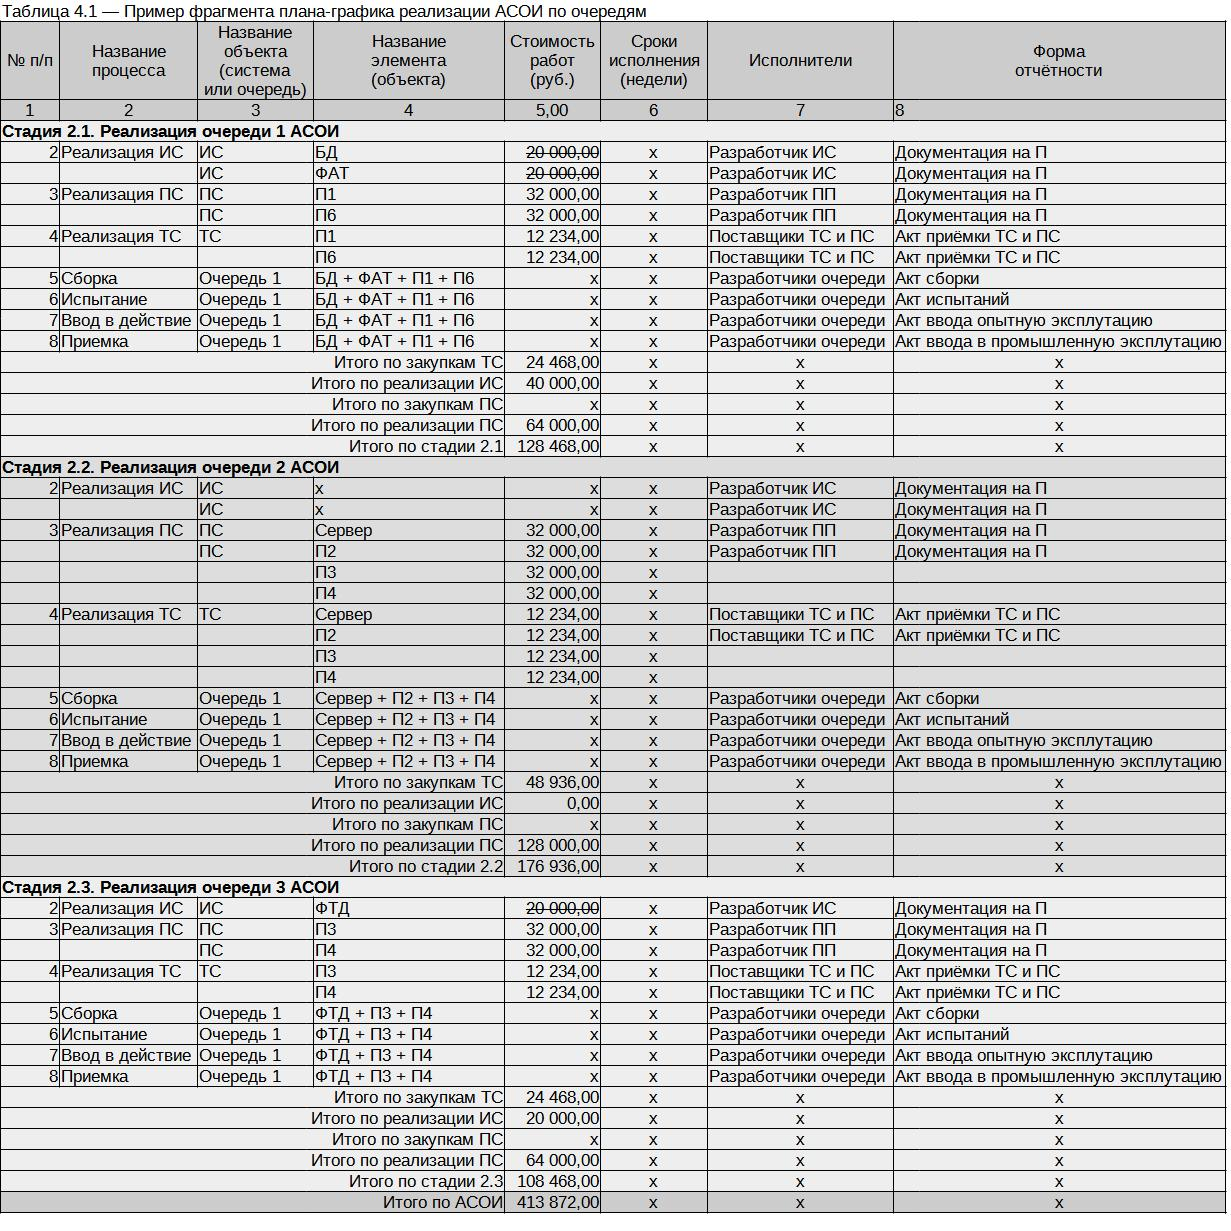
\includegraphics[width=16cm]
            {_docs/Таблица4-1ПримерФрагментаПлана-графикаРеализацииАСОИПоОчередям.jpg}
        \caption{Пример фрагмента плана-графика реализации АСОИ по очередям}
    \end{figure}

\end{document}
